In Chapter~\ref{zop} we used a tuned LC circuit placed directly above the processor's bypass capacitors as a probe to receive the modulated processor clock signal at $f_c = 50$ MHz. In this chapter we use a processor clock frequency of $f_c = 83.333$ MHz. The signal received with this setup is very strong and essentially free from noise and interferences. However, at this frequency and distance, the probe is in the near field and so the received signal decays quickly as the distance is increased, so that at a distance of a few centimeters the signal amplitude is too low to be used. At the processor frequency (83.333 MHz), our target distance (3 meters) is still not in the far field and so a sophisticated (and likely very large) near field probe would be needed to provide a strong enough signal. The processor and memory clocks are roughly square waves, and so EM emanations are generated at the harmonics (multiples) of the processor clock frequency. As the frequency increases the minimum far field distance decreases and compact high gain antennas can be used, so we will attempt to demodulate and characterize these clock harmonics. 

Before using ZOP at a distance, we characterized the signals ZOP uses, focusing on the signal effects which change as a function of the distance, antenna, and the harmonic used. First, we characterized the strength of the carriers and modulated signals generated at the harmonics of the processor clock. To do this, we first need a modulation signal (i.e. system activity) which is easy to control and measure. The LDM/LDL1 (Load from Memory vs Load from L1 Cache) SAVAT benchmark generates a narrow peak in the sideband of all the carriers modulated by this activity. In this experiment, modulated carriers exist at all the harmonics of the processor clock (e.g. the first harmonic at 83.333 MHz, the second harmonic at 166.666 MHz, etc.). For each of these carriers, we made 6 measurements. First we measured the power of the signal generated at the carrier, where the carrier occurs at frequency $f_h = h f_1$ where $f_1 = 83.333$ MHz. Then we measured the power of the SAVAT modulation signal occurring in the right and left sidebands at $f_h \pm f_{alt}$ where $f_{alt} = 100$ kHz (the SAVAT alternation frequency). The power is integrated across a 10 kHz band centered at the frequency of interest to allow for any spread or variation in the frequency of the generated sidebands. First we do each of these measurements with the FPGA powered on and SAVAT running. Next, we power off the FPGA and remeasure the signal power at $f_h, f_h - f_{alt}, f_h + f_{alt}$ again to get an indication of the ambient noise at these frequencies. We performed each of these measurements at the harmonics from $h = 1$ (83.333 MHz) to $h = 43$ (3.5833 GHz). We use a Com-Power AH-118 broadband double ridge horn antenna, which has a relatively flat frequency response from 700 MHz to 18 GHz and 10 dBi gain over this frequency range. The signal was recorded using the same N9020A MXA spectrum analyzer as in previous experiments. The distance between the FPGA board and the antenna was 60 cm.

In Figure~\ref{savat_harm_mag}, each line shows the power measured at the carrier and sideband frequencies with SAVAT active minus the power at these same frequencies with the FPGA powered off. Note that we can only measure these quantities at the frequencies that are harmonics of the clock, so for each trace, there are 43 evenly spaced data points (for harmonics $h = 1$ to $h = 43$). A line is drawn connecting these points to indicate the general trend in power as a function frequency. As shown in the figure, the left and right sidebands have comparable powers. This is expected because the distance between the right and left alternation frequency is only $2 f_{alt} = 200$ kHz and the frequency response of the channel is expected to be flat over such a narrow span. The power of the SAVAT signals is approximately 20 dB above the noise floor for most frequencies, indicating a strong (usable) signal exists at many harmonics. Most interestingly, the power of the carriers and sidebands does not decay significantly as frequency increases. While the higher order harmonics of an ideal square wave decay quickly as a function of frequency, the signal received in this setup is affected by several additional factors. First, the currents and voltages generated within the FPGA, DRAM, and PCB at the carrier and modulation frequencies will vary greatly as a function of frequency. Also, for a current of a given magnitude flowing through a wire on a PCB, a stronger EM field will be generated as the frequency of the current increases. 

\begin{figure}[hbt]
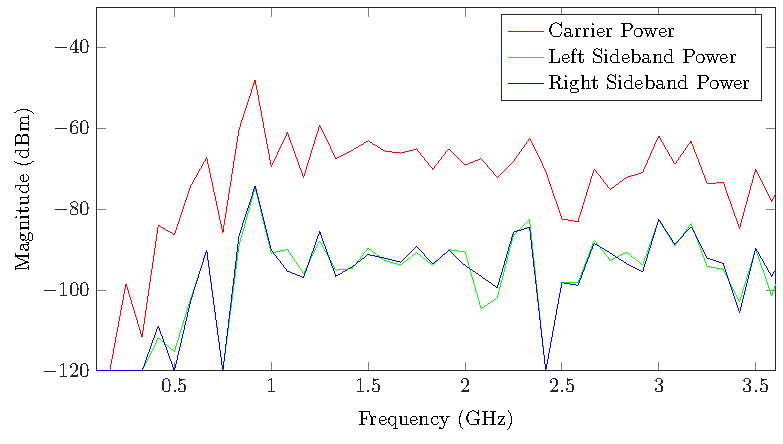
\includegraphics[width=5in]{savat_harm_mag}
\caption{Magnitude of processor clock harmonics 1 through 43 as carriers and as modulated by 100 KHz SAVAT LDM/LDL1 activity.}
\label{savat_harm_mag}
\end{figure}

To reliably receive the signals ZOP uses, we need to pick a frequency range where antennas with high gain can be found. We chose the 2.3 GHz - 2.7 GHz frequency range because it is widely used for wifi and other wireless protocols, and so many high gain commercial antennas are available. For several antenna types and carriers (harmonics) in this range we measured the EM emanations while executing the replace benchmark repeatedly with the same inputs. In Chapter~\ref{zop} we found that simple AM demodulation (i.e. simply taking the magnitude of of the IQ signal for the 8.333 MHz band around the carrier) resulted in a very strong signal with very little noise when using the tuned LC inductor probe at 83.333 MHz. Repeated executions of the benchmark for this setup resulted in demodulated waveforms with almost no noise, so that there was very little signal variation between repeated executions of a program with the same inputs. However, when we demodulated the harmonics similarly with several different types of antennas and frequencies in the 2.3 GHz - 2.7 GHz band, we found that there was little relation between the SAVAT power in Figure~\ref{savat_harm_mag} and the signal strength in demodulated waveforms for a given frequency and antenna. 

This variation in the signal strength relative to SAVAT power was determined to be caused by the nature of the unintentional modulation of signals within computer systems. In modern communications systems, the transmitter minimizes the power wasted on the continuous wave carrier to order to maximize the power available to modulate the carrier and transmit information. Furthermore, the phase and magnitude of the transmitted signals are carefully controlled to maximize data transfer rates. Unintentionally modulated computing signals (such as processor clocks) are not designed as carriers, and so do not have either of these two properties. First, a large portion of the transmitted power is not modulated. For example, the power consumed by a processor as it executes a program may vary during different portions of a program, but there is a non-zero minimum amount of power consumed by the circuitry on the processor clock, and this minimum can be on the order of the variations in power usage over the execution of a program. Second, different circuitry driven by the same clock may not all share a common phase (for example there may be a phase difference between the processor and memory activities even when they share the same clock), and similarly it is plausible that delays through the power distribution network could result in phase variation in the current drawn (and therefore cause phase variations in the EM emanations). 

%could potentially have additional sources (maybe show example)

Previously we used asynchronous AM demodulation, but to understand these modulation effects we first applied carrier recovery to compensate for the small frequency offset between the receiver (the spectrum analyzer) and transmitter (the computing device under test). After this, the unexplained variation in the signal strength was obvious and can be explained by Figure~\ref{multiple_clock_components}. We hypothesize that the EM emanations from a computing device can be modeled as $s(t) = C e^{jwt} + M(t) e^{j\cdot(wt+\phi)}$ where the first component $C e^{jwt}$ is a sinusoid at the carrier frequency $w$ with real magnitude $C$ and the second component $M(t) e^{j\cdot(wt+\phi)}$ is at the same carrier frequency $w$ but has modulated magnitude $M(t)$ and a phase offset $\phi$ relative to the first component. Based on these assumptions, after carrier recovery (e.g. in the simplest form, multiplying $s(t)$ by $e^{-jwt}$) we would expect the AM modulated component to be offset from the origin by $C$ and rotated by $\phi$ in an IQ plot. Figure~\ref{all_iq_h31} shows IQ plots for demodulated signals after carrier recovery for the 31st harmonic at 2.58 GHz with several antennas and antenna orientations. The upper left plot shows the demodulated data for a H field probe placed directly on top of the FPGA. The remaining plots were measured at a distance of 60 cm. The bottom left plot shows results for a helical antenna. The other plots show results for the same 10 dBi horn antenna used before, and an L-com HG2418P 2.4 GHz 18 dBi directional panel antenna, with two plots each showing two orthogonal orientations. For each of these measurements, a low noise amplifier with a 1 dB noise figure and 20 dB of gain was placed between the antenna and spectrum analyzer. Each dot in a plot represents an IQ sample in the demodulated waveform recorded during execution of the replace benchmark with the same inputs after carrier recovery. The large red X marks the origin (i.e. $I=0, Q=0$). The mean IQ value across all the samples for a given plot is different in each plot, and the dominant variation axis is rotated by varying angles between the plots. These results agree with the hypothesis that the EM emanations at the processor/memory clock frequency consists of two components: one unmodulated, and one modulated and rotated by angle $\phi$.

\begin{figure}[hbt]
\includegraphics[width=5in]{multiple_clock_components}
\caption{A diagram illustrating an IQ plot for an unintentionally modulated signal with two synchronous components (one modulated, one not modulated) with the same frequency but different phases.}
\label{multiple_clock_components}
\end{figure}

\begin{figure*}
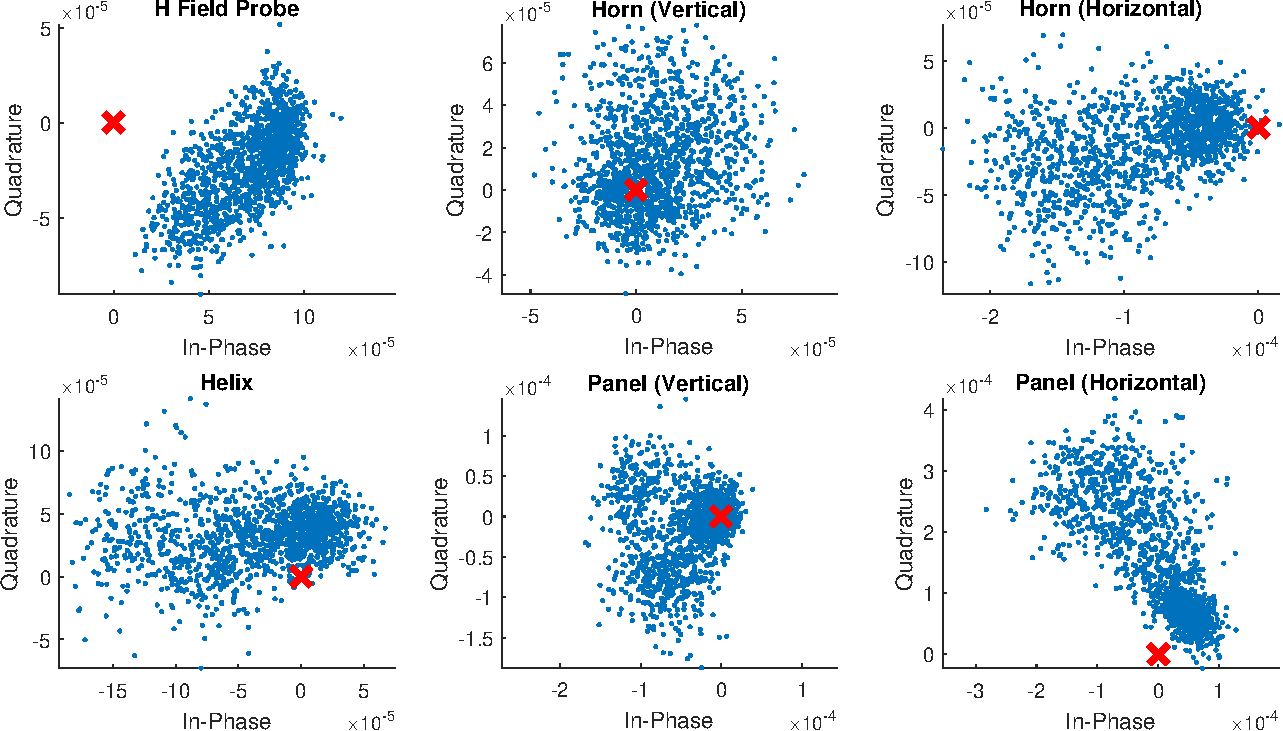
\includegraphics[width=\textwidth]{all_iq_h31}
\caption{IQ plots for the modulated 31st clock harmonic with several antennas and orientations.}
\label{all_iq_h31}
\end{figure*}

Based on these measurements and analysis it is clear why the demodulated signal strength is not directly related to the measured SAVAT power. Depending on the phase offset $\phi$, more or less of the signal is captured by AM demodulation. For example, as shown in Figure~\ref{all_iq_h31}, if we demodulate by simply taking the magnitude of each IQ sample we will capture a small fraction of the signal when using the H field probe signal but will capture a much larger (though still not optimal) fraction of the signal for the helical antenna. It is important to note that some portion of the signal is present in the variation orthogonal to the main axis of modulation. In other words the signal is phase modulated in addition to being AM modulated. Regardless of the choice of offset and axis for AM demodulation, repeatable patterns are present in the phase of the IQ samples as a function of time across repeated executions of the same program and inputs. Therefore AM demodulating the signal throws away some usable signal. This repeatable phase variation might be explained by the fact that there are many small circuits drawing current with slightly different phases when they are active resulting not only a continuous range of amplitudes but also a continuous range of possible phases. It is also likely that the channel's frequency response is not completely flat. This can contribute to repeatable phase variation even for purely AM modulated signals. %For example, we might expect no signal or pattern in the phase as a function of time after doing simple AM demodulation of the signal show in the IQ plot for the horn antenna in the horizontal orientation. However, Figure~\ref{

\begin{figure*}
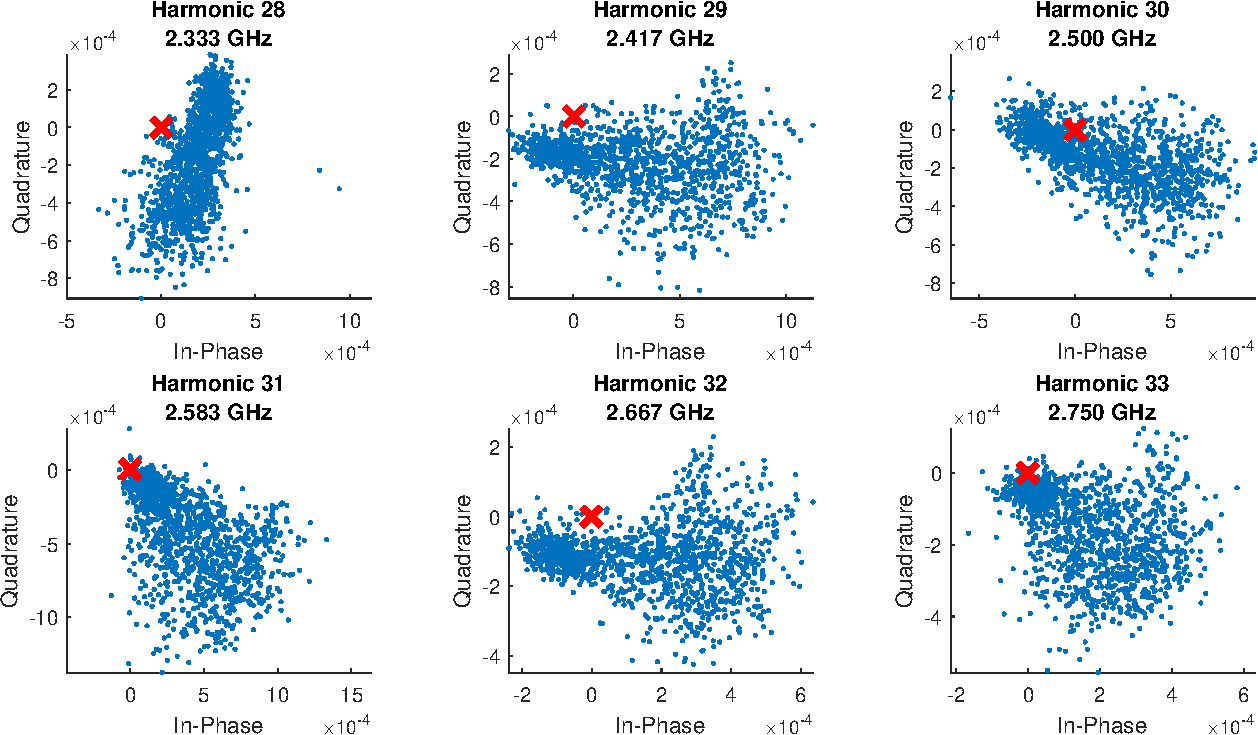
\includegraphics[width=\textwidth]{panel_iq_hx}
\caption{IQ plots for several harmonics using the 18 dBi panel antenna with horizontal orientation.}
\label{panel_iq_hx}
\end{figure*}

It is also interesting to compare IQ plots for multiple harmonics of the same processor clock signal. Figure~\ref{panel_iq_hx} shows IQ plots for several such harmonics using the same panel antenna at a distance of 60 cm. In terms of the demodulated waveform shape in the time domain, from theory we would expect the demodulated signals from different harmonics of the same clock to have the same shape. Figure~\ref{panel_abs_hx} shows that this is largely true. This is significant because it suggests signals from multiple harmonics can be combined together to increase the signal strength and to overcome interferences in individual harmonics. 

\begin{figure*}
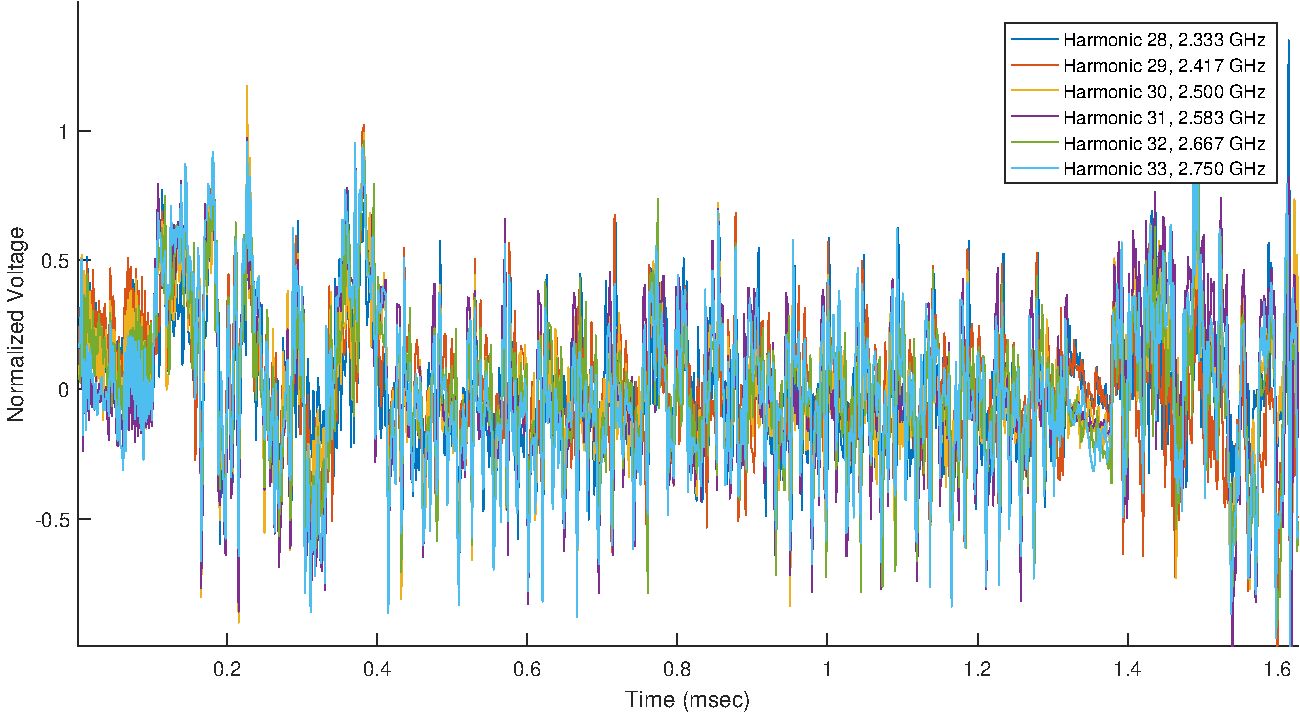
\includegraphics[width=\textwidth]{panel_abs_hx}
\caption{Demodulated and normalized time domain signals for several harmonics using the 18 dBi panel antenna with horizontal orientation.}
\label{panel_abs_hx}
\end{figure*}

Finally, we are interested in how the signal decays with distance. Figure~\ref{panel_abs_h31_cm} overlays the demodulated time domain signal for 10 repeated executions of the same benchmark with the same inputs for the 31st harmonic, comparing the waveform shape at 60 cm and 300 cm. While the signal magnitude is slightly lower at 300 cm, the overall waveform shape is similar for these two distances. 

\begin{figure*}
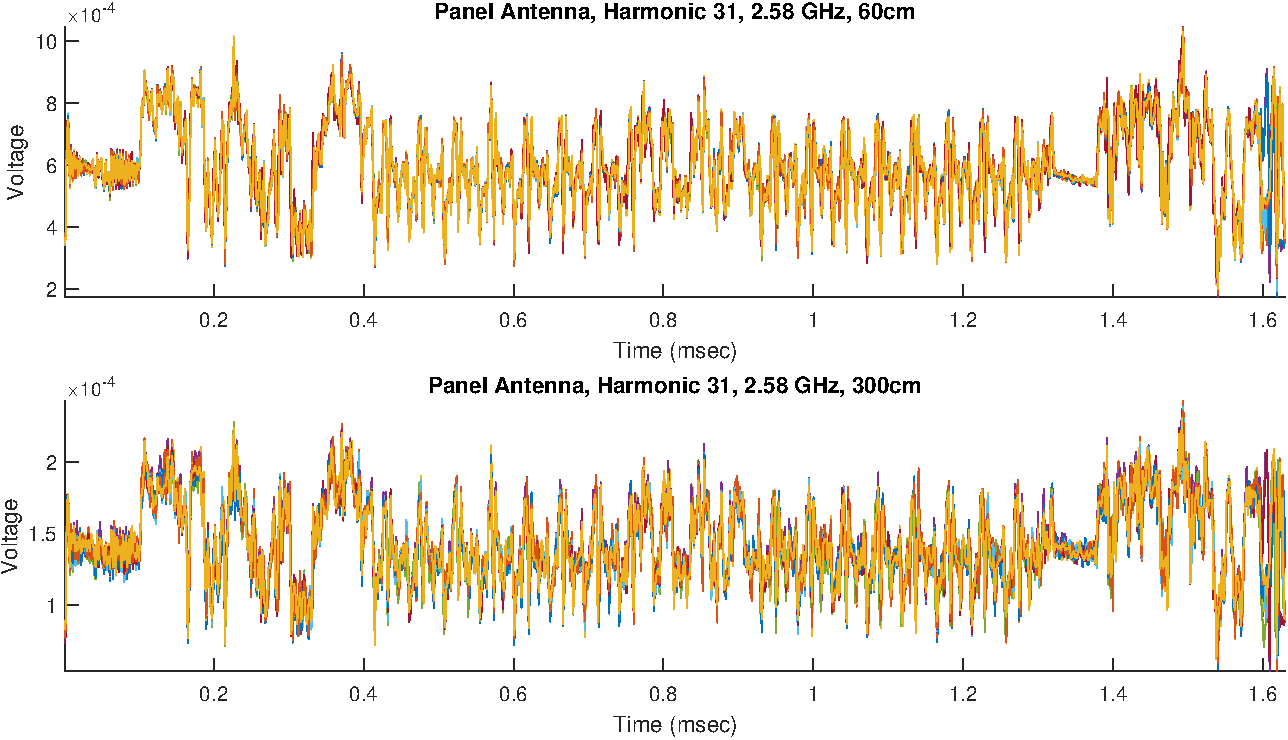
\includegraphics[width=\textwidth]{panel_abs_h31_cm}
\caption{IQ plots for 10 repeated runs of the same benchmark and inputs for the 31st harmonic at 60 cm (top) and 300 cm (bottom)  using the 18 dBi panel antenna with horizontal orientation.}
\label{panel_abs_h31_cm}
\end{figure*}

%carrier tracking
%removing complex offset

In order to begin to understand how signal quality for a given environment (i.e. antenna, amplifier, distance, etc.) can affect ZOP's performance, we first need a metric to quantify the ``usable'' signal strength. Some methods for quantifying average signal strength require significant control over the signals generated by the transmitter, or theoretical assumptions about the transmitter. It is not obvious how to apply these methods to our scenario, as the only control we have is the ability to generate the same pattern repeatedly by executing the same benchmark with the same inputs and observing variation in this signal. Any feature of the received signal which is common between all the repeated executions (i.e. present in the mean across all the executions at a given time point) will be referred to as ``positively correlated'' since these features contribute to higher correlation between any two waveforms measured during repeated execution of the same code (assuming the waveforms are normalized). Any feature in the signal which is present in a single execution but not present in the mean across all repeated executions will be considered ``negatively correlated'' since such features tend to contribute to lower correlation between two waveforms measured during repeated execution of the same code.

We next define a single value that represents the average strength (magnitude) for a newly defined signal consisting of the sum of all the positively correlated features in a given set of waveforms measured during repeated executions of the same code (call this value $P$), and similarly define a single value for the average magnitude of the signal consisting of the sum of the negatively correlated features (call this value $N$). If $x[r,t]$ is the (demodulated) signal value at time $t$ of the $r$th repeated execution, then we can estimate $P$ by first taking the mean among all the repeated waveforms $x[r,t]$ at each time instant $t$ to create an average signal $p[t]$ and then taking the standard deviation of $p[t]$ across all time $t$:
\begin{equation}
\begin{aligned}
p[t] &= \textrm{mean}_r \> x[r,t] \\
P &= \textrm{std} \> p[t].
\end{aligned}
\end{equation}
$P$ is then a single value that estimates of the magnitude of the signal that is common between executions. Similarly, we can estimate $N$ as
\begin{equation}
% 2/15/2017: changed t -> r. take std() of each waveform, then mean of these stds(). same as in slides and matlab code
\begin{aligned}
n[r] &= \textrm{std}_t \> (x[r,t] - p[t]) \\
N &= \textrm{mean} \> n[r].
\end{aligned}
\end{equation}
Then a given program execution $r$ has a waveform $x[r,t]$ which can be decomposed into two signals: $p[t]$ (the signal consisting of the positively correlated features which are common between all executions) and $x[r,t] - p[t]$ (the signal consisting of the negatively correlated features present in $x[r,t]$ but in present among all the other executions). 

\begin{figure}[hbt]
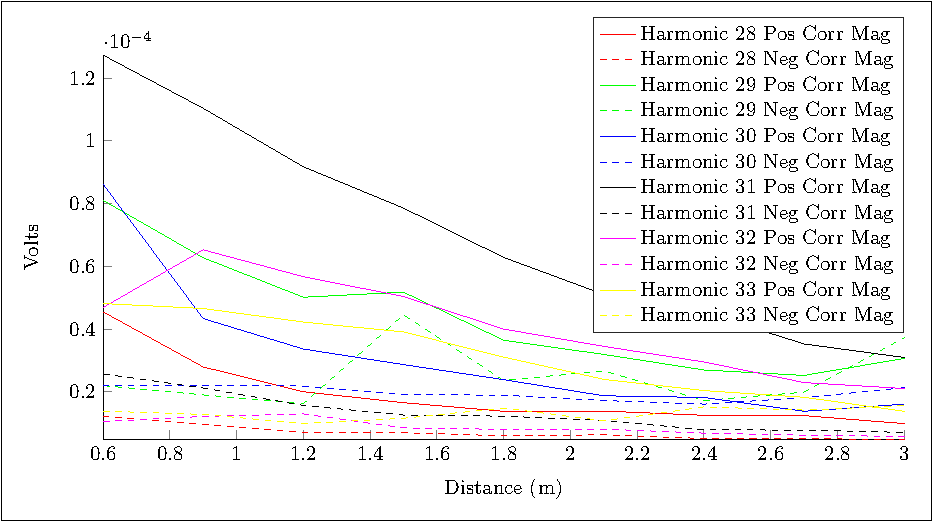
\includegraphics[width=5in]{snr_distance}
\caption{A plot of the magnitudes of the positively and negatively correlated signal features as a function of distance using 18 dBi panel antenna with horizontal orientation.}
\label{snr_distance}
\end{figure}

\begin{figure}[hbt]
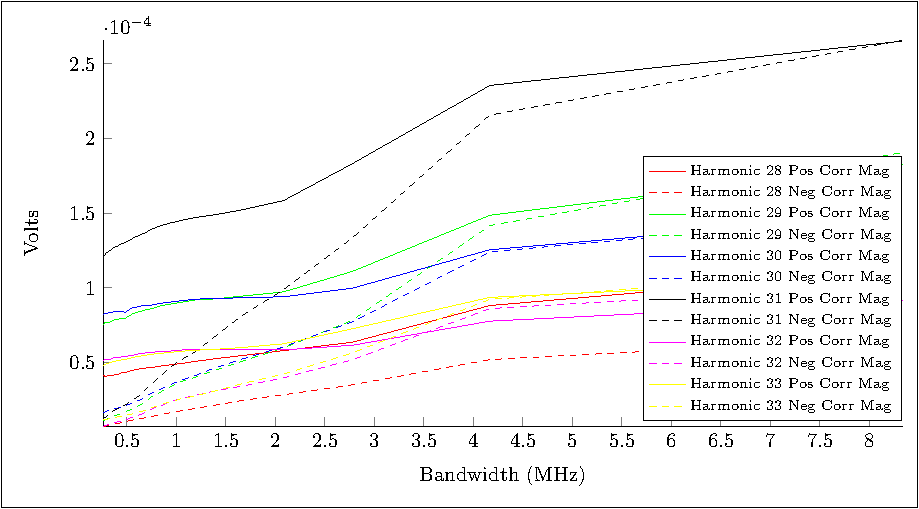
\includegraphics[width=5in]{snr_bandwidth}
\caption{A plot of the magnitudes of the positively and negatively correlated signal features as a function of demodulation bandwidth using 18 dBi panel antenna with horizontal orientation.}
\label{snr_bandwidth}
\end{figure}


One usage of the $P$ and $N$ values is to estimate the decay of the signal as a function of distance. This is shown in Figure~\ref{snr_distance}. In the figure, the magnitude of the negatively correlated features, $N$, is constant for a given harmonic, as would be expected for a fixed level of ambient noise. This figure also confirms that simple AM demodulation captures only a varying portion of the total signal depending on the complex offset $C$ introduced by the non-modulated component in the IQ plot together with the phase rotation $\phi$. For example, in Figure~\ref{panel_iq_hx}, the 28th harmonic has a complex offset $C$ and phase $\phi$ that results in the least fraction of the total signal being captured by simple AM demodulation, and also has the lowest signal level in Figure~\ref{snr_distance}. Similarly, the 31th harmonic's complex offset $C$ is the smallest, resulting the strongest signal level in Figure~\ref{snr_distance}. In the IQ plots in Figure~\ref{panel_iq_hx}, the area with the highest concentration of samples corresponds to the point where the modulation signal $M(t)$ is at its minimum. For these signals subtracting this offset before AM demodulating would yield the strongest signal, i.e. the signal with the largest $P/N$ value.

Figure~\ref{snr_bandwidth} shows the magnitudes of the positively and negatively correlated signal features as a function of the demodulation bandwidth (i.e. the width of the frequency band around the carrier that is demodulated) for the same demodulated harmonics and measurement setup used for Figures~\ref{panel_iq_hx} and~\ref{snr_distance}. This figure shows that the ratio $P/N$ is in fact lower at higher baseband frequencies, meaning that as we increase the demodulation bandwidth, we would expect the correlation between the training waveforms and the to-be-predicted waveforms to decrease. We confirmed this by using ZOP with different demodulation bandwidths and observing that if the bandwidth was too high, the performance suffered. The fact that $P/N$ decreases as frequency increases suggests that there is increasing time and/or amplitude variation in the waveform features generated for very rapid changes in processor activity. One explanation for this phenomenon is that for repeated executions of the same program with the same inputs, the variation in microarchitectural activity occurs on small timescales, generating high frequency features in the signal, but that it is much more difficult for microarchitectural activity to cause low frequency features. This makes intuitive sense because it is extremely unlikely that microarchitectural variation alone could cause a program to take 1 second for one execution and 2 seconds for another run of the same program, but it is plausible that microarchitectural activity could cause a section of code to take 100 clock cycles in one execution vs 200 clock cycles in another execution. 






